% Created by tikzDevice version 0.10.1 on 2017-11-22 16:44:33
% !TEX encoding = UTF-8 Unicode
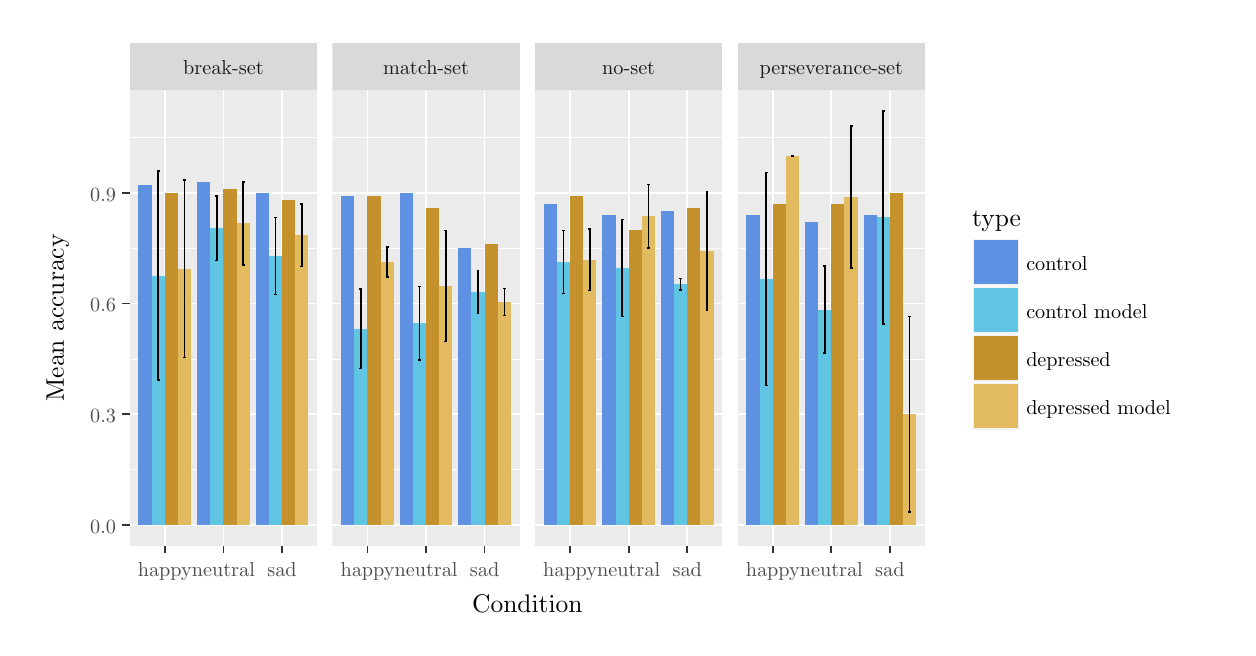
\begin{tikzpicture}[x=1pt,y=1pt]
\definecolor{fillColor}{RGB}{255,255,255}
\path[use as bounding box,fill=fillColor,fill opacity=0.00] (0,0) rectangle (433.62,216.81);
\begin{scope}
\path[clip] (  0.00,  0.00) rectangle (433.62,216.81);
\definecolor{drawColor}{RGB}{255,255,255}
\definecolor{fillColor}{RGB}{255,255,255}

\path[draw=drawColor,line width= 0.6pt,line join=round,line cap=round,fill=fillColor] (  0.00,  0.00) rectangle (433.62,216.81);
\end{scope}
\begin{scope}
\path[clip] ( 36.87, 29.59) rectangle (104.59,194.25);
\definecolor{fillColor}{gray}{0.92}

\path[fill=fillColor] ( 36.87, 29.59) rectangle (104.59,194.25);
\definecolor{drawColor}{RGB}{255,255,255}

\path[draw=drawColor,line width= 0.3pt,line join=round] ( 36.87, 57.08) --
	(104.59, 57.08);

\path[draw=drawColor,line width= 0.3pt,line join=round] ( 36.87, 97.11) --
	(104.59, 97.11);

\path[draw=drawColor,line width= 0.3pt,line join=round] ( 36.87,137.13) --
	(104.59,137.13);

\path[draw=drawColor,line width= 0.3pt,line join=round] ( 36.87,177.16) --
	(104.59,177.16);

\path[draw=drawColor,line width= 0.6pt,line join=round] ( 36.87, 37.07) --
	(104.59, 37.07);

\path[draw=drawColor,line width= 0.6pt,line join=round] ( 36.87, 77.10) --
	(104.59, 77.10);

\path[draw=drawColor,line width= 0.6pt,line join=round] ( 36.87,117.12) --
	(104.59,117.12);

\path[draw=drawColor,line width= 0.6pt,line join=round] ( 36.87,157.15) --
	(104.59,157.15);

\path[draw=drawColor,line width= 0.6pt,line join=round] ( 49.56, 29.59) --
	( 49.56,194.25);

\path[draw=drawColor,line width= 0.6pt,line join=round] ( 70.73, 29.59) --
	( 70.73,194.25);

\path[draw=drawColor,line width= 0.6pt,line join=round] ( 91.89, 29.59) --
	( 91.89,194.25);
\definecolor{fillColor}{RGB}{226,186,95}

\path[fill=fillColor] ( 54.33, 37.07) rectangle ( 59.09,129.65);
\definecolor{fillColor}{RGB}{196,145,45}

\path[fill=fillColor] ( 49.56, 37.07) rectangle ( 54.33,157.15);
\definecolor{fillColor}{RGB}{95,197,226}

\path[fill=fillColor] ( 44.80, 37.07) rectangle ( 49.56,127.21);
\definecolor{fillColor}{RGB}{95,145,226}

\path[fill=fillColor] ( 40.04, 37.07) rectangle ( 44.80,159.81);
\definecolor{fillColor}{RGB}{226,186,95}

\path[fill=fillColor] ( 75.49, 37.07) rectangle ( 80.25,146.11);
\definecolor{fillColor}{RGB}{196,145,45}

\path[fill=fillColor] ( 70.73, 37.07) rectangle ( 75.49,158.48);
\definecolor{fillColor}{RGB}{95,197,226}

\path[fill=fillColor] ( 65.97, 37.07) rectangle ( 70.73,144.38);
\definecolor{fillColor}{RGB}{95,145,226}

\path[fill=fillColor] ( 61.20, 37.07) rectangle ( 65.97,161.15);
\definecolor{fillColor}{RGB}{226,186,95}

\path[fill=fillColor] ( 96.65, 37.07) rectangle (101.41,141.77);
\definecolor{fillColor}{RGB}{196,145,45}

\path[fill=fillColor] ( 91.89, 37.07) rectangle ( 96.65,154.48);
\definecolor{fillColor}{RGB}{95,197,226}

\path[fill=fillColor] ( 87.13, 37.07) rectangle ( 91.89,134.27);
\definecolor{fillColor}{RGB}{95,145,226}

\path[fill=fillColor] ( 82.37, 37.07) rectangle ( 87.13,157.15);
\definecolor{drawColor}{RGB}{0,0,0}

\path[draw=drawColor,line width= 0.6pt,line join=round] ( 56.18,161.67) --
	( 57.24,161.67);

\path[draw=drawColor,line width= 0.6pt,line join=round] ( 56.71,161.67) --
	( 56.71, 97.64);

\path[draw=drawColor,line width= 0.6pt,line join=round] ( 56.18, 97.64) --
	( 57.24, 97.64);

\path[draw=drawColor,line width= 0.6pt,line join=round] ( 46.65,164.99) --
	( 47.71,164.99);

\path[draw=drawColor,line width= 0.6pt,line join=round] ( 47.18,164.99) --
	( 47.18, 89.42);

\path[draw=drawColor,line width= 0.6pt,line join=round] ( 46.65, 89.42) --
	( 47.71, 89.42);

\path[draw=drawColor,line width= 0.6pt,line join=round] ( 77.34,161.13) --
	( 78.40,161.13);

\path[draw=drawColor,line width= 0.6pt,line join=round] ( 77.87,161.13) --
	( 77.87,131.08);

\path[draw=drawColor,line width= 0.6pt,line join=round] ( 77.34,131.08) --
	( 78.40,131.08);

\path[draw=drawColor,line width= 0.6pt,line join=round] ( 67.82,156.10) --
	( 68.88,156.10);

\path[draw=drawColor,line width= 0.6pt,line join=round] ( 68.35,156.10) --
	( 68.35,132.66);

\path[draw=drawColor,line width= 0.6pt,line join=round] ( 67.82,132.66) --
	( 68.88,132.66);

\path[draw=drawColor,line width= 0.6pt,line join=round] ( 98.50,153.00) --
	( 99.56,153.00);

\path[draw=drawColor,line width= 0.6pt,line join=round] ( 99.03,153.00) --
	( 99.03,130.53);

\path[draw=drawColor,line width= 0.6pt,line join=round] ( 98.50,130.53) --
	( 99.56,130.53);

\path[draw=drawColor,line width= 0.6pt,line join=round] ( 88.98,148.17) --
	( 90.04,148.17);

\path[draw=drawColor,line width= 0.6pt,line join=round] ( 89.51,148.17) --
	( 89.51,120.37);

\path[draw=drawColor,line width= 0.6pt,line join=round] ( 88.98,120.37) --
	( 90.04,120.37);
\end{scope}
\begin{scope}
\path[clip] (110.09, 29.59) rectangle (177.81,194.25);
\definecolor{fillColor}{gray}{0.92}

\path[fill=fillColor] (110.09, 29.59) rectangle (177.81,194.25);
\definecolor{drawColor}{RGB}{255,255,255}

\path[draw=drawColor,line width= 0.3pt,line join=round] (110.09, 57.08) --
	(177.81, 57.08);

\path[draw=drawColor,line width= 0.3pt,line join=round] (110.09, 97.11) --
	(177.81, 97.11);

\path[draw=drawColor,line width= 0.3pt,line join=round] (110.09,137.13) --
	(177.81,137.13);

\path[draw=drawColor,line width= 0.3pt,line join=round] (110.09,177.16) --
	(177.81,177.16);

\path[draw=drawColor,line width= 0.6pt,line join=round] (110.09, 37.07) --
	(177.81, 37.07);

\path[draw=drawColor,line width= 0.6pt,line join=round] (110.09, 77.10) --
	(177.81, 77.10);

\path[draw=drawColor,line width= 0.6pt,line join=round] (110.09,117.12) --
	(177.81,117.12);

\path[draw=drawColor,line width= 0.6pt,line join=round] (110.09,157.15) --
	(177.81,157.15);

\path[draw=drawColor,line width= 0.6pt,line join=round] (122.79, 29.59) --
	(122.79,194.25);

\path[draw=drawColor,line width= 0.6pt,line join=round] (143.95, 29.59) --
	(143.95,194.25);

\path[draw=drawColor,line width= 0.6pt,line join=round] (165.11, 29.59) --
	(165.11,194.25);
\definecolor{fillColor}{RGB}{226,186,95}

\path[fill=fillColor] (127.55, 37.07) rectangle (132.31,132.20);
\definecolor{fillColor}{RGB}{196,145,45}

\path[fill=fillColor] (122.79, 37.07) rectangle (127.55,155.81);
\definecolor{fillColor}{RGB}{95,197,226}

\path[fill=fillColor] (118.02, 37.07) rectangle (122.79,108.05);
\definecolor{fillColor}{RGB}{95,145,226}

\path[fill=fillColor] (113.26, 37.07) rectangle (118.02,155.81);
\definecolor{fillColor}{RGB}{226,186,95}

\path[fill=fillColor] (148.71, 37.07) rectangle (153.47,123.47);
\definecolor{fillColor}{RGB}{196,145,45}

\path[fill=fillColor] (143.95, 37.07) rectangle (148.71,151.81);
\definecolor{fillColor}{RGB}{95,197,226}

\path[fill=fillColor] (139.19, 37.07) rectangle (143.95,110.03);
\definecolor{fillColor}{RGB}{95,145,226}

\path[fill=fillColor] (134.43, 37.07) rectangle (139.19,157.15);
\definecolor{fillColor}{RGB}{226,186,95}

\path[fill=fillColor] (169.87, 37.07) rectangle (174.64,117.70);
\definecolor{fillColor}{RGB}{196,145,45}

\path[fill=fillColor] (165.11, 37.07) rectangle (169.87,138.47);
\definecolor{fillColor}{RGB}{95,197,226}

\path[fill=fillColor] (160.35, 37.07) rectangle (165.11,121.37);
\definecolor{fillColor}{RGB}{95,145,226}

\path[fill=fillColor] (155.59, 37.07) rectangle (160.35,137.13);
\definecolor{drawColor}{RGB}{0,0,0}

\path[draw=drawColor,line width= 0.6pt,line join=round] (129.40,137.57) --
	(130.46,137.57);

\path[draw=drawColor,line width= 0.6pt,line join=round] (129.93,137.57) --
	(129.93,126.83);

\path[draw=drawColor,line width= 0.6pt,line join=round] (129.40,126.83) --
	(130.46,126.83);

\path[draw=drawColor,line width= 0.6pt,line join=round] (119.88,122.40) --
	(120.93,122.40);

\path[draw=drawColor,line width= 0.6pt,line join=round] (120.40,122.40) --
	(120.40, 93.70);

\path[draw=drawColor,line width= 0.6pt,line join=round] (119.88, 93.70) --
	(120.93, 93.70);

\path[draw=drawColor,line width= 0.6pt,line join=round] (150.56,143.49) --
	(151.62,143.49);

\path[draw=drawColor,line width= 0.6pt,line join=round] (151.09,143.49) --
	(151.09,103.45);

\path[draw=drawColor,line width= 0.6pt,line join=round] (150.56,103.45) --
	(151.62,103.45);

\path[draw=drawColor,line width= 0.6pt,line join=round] (141.04,123.28) --
	(142.10,123.28);

\path[draw=drawColor,line width= 0.6pt,line join=round] (141.57,123.28) --
	(141.57, 96.77);

\path[draw=drawColor,line width= 0.6pt,line join=round] (141.04, 96.77) --
	(142.10, 96.77);

\path[draw=drawColor,line width= 0.6pt,line join=round] (171.73,122.61) --
	(172.78,122.61);

\path[draw=drawColor,line width= 0.6pt,line join=round] (172.25,122.61) --
	(172.25,112.79);

\path[draw=drawColor,line width= 0.6pt,line join=round] (171.73,112.79) --
	(172.78,112.79);

\path[draw=drawColor,line width= 0.6pt,line join=round] (162.20,128.96) --
	(163.26,128.96);

\path[draw=drawColor,line width= 0.6pt,line join=round] (162.73,128.96) --
	(162.73,113.79);

\path[draw=drawColor,line width= 0.6pt,line join=round] (162.20,113.79) --
	(163.26,113.79);
\end{scope}
\begin{scope}
\path[clip] (183.31, 29.59) rectangle (251.03,194.25);
\definecolor{fillColor}{gray}{0.92}

\path[fill=fillColor] (183.31, 29.59) rectangle (251.03,194.25);
\definecolor{drawColor}{RGB}{255,255,255}

\path[draw=drawColor,line width= 0.3pt,line join=round] (183.31, 57.08) --
	(251.03, 57.08);

\path[draw=drawColor,line width= 0.3pt,line join=round] (183.31, 97.11) --
	(251.03, 97.11);

\path[draw=drawColor,line width= 0.3pt,line join=round] (183.31,137.13) --
	(251.03,137.13);

\path[draw=drawColor,line width= 0.3pt,line join=round] (183.31,177.16) --
	(251.03,177.16);

\path[draw=drawColor,line width= 0.6pt,line join=round] (183.31, 37.07) --
	(251.03, 37.07);

\path[draw=drawColor,line width= 0.6pt,line join=round] (183.31, 77.10) --
	(251.03, 77.10);

\path[draw=drawColor,line width= 0.6pt,line join=round] (183.31,117.12) --
	(251.03,117.12);

\path[draw=drawColor,line width= 0.6pt,line join=round] (183.31,157.15) --
	(251.03,157.15);

\path[draw=drawColor,line width= 0.6pt,line join=round] (196.01, 29.59) --
	(196.01,194.25);

\path[draw=drawColor,line width= 0.6pt,line join=round] (217.17, 29.59) --
	(217.17,194.25);

\path[draw=drawColor,line width= 0.6pt,line join=round] (238.33, 29.59) --
	(238.33,194.25);
\definecolor{fillColor}{RGB}{226,186,95}

\path[fill=fillColor] (200.77, 37.07) rectangle (205.53,132.96);
\definecolor{fillColor}{RGB}{196,145,45}

\path[fill=fillColor] (196.01, 37.07) rectangle (200.77,155.81);
\definecolor{fillColor}{RGB}{95,197,226}

\path[fill=fillColor] (191.25, 37.07) rectangle (196.01,132.15);
\definecolor{fillColor}{RGB}{95,145,226}

\path[fill=fillColor] (186.48, 37.07) rectangle (191.25,153.14);
\definecolor{fillColor}{RGB}{226,186,95}

\path[fill=fillColor] (221.93, 37.07) rectangle (226.69,148.65);
\definecolor{fillColor}{RGB}{196,145,45}

\path[fill=fillColor] (217.17, 37.07) rectangle (221.93,143.80);
\definecolor{fillColor}{RGB}{95,197,226}

\path[fill=fillColor] (212.41, 37.07) rectangle (217.17,129.98);
\definecolor{fillColor}{RGB}{95,145,226}

\path[fill=fillColor] (207.65, 37.07) rectangle (212.41,149.14);
\definecolor{fillColor}{RGB}{226,186,95}

\path[fill=fillColor] (243.10, 37.07) rectangle (247.86,136.02);
\definecolor{fillColor}{RGB}{196,145,45}

\path[fill=fillColor] (238.33, 37.07) rectangle (243.10,151.81);
\definecolor{fillColor}{RGB}{95,197,226}

\path[fill=fillColor] (233.57, 37.07) rectangle (238.33,124.16);
\definecolor{fillColor}{RGB}{95,145,226}

\path[fill=fillColor] (228.81, 37.07) rectangle (233.57,150.47);
\definecolor{drawColor}{RGB}{0,0,0}

\path[draw=drawColor,line width= 0.6pt,line join=round] (202.62,144.11) --
	(203.68,144.11);

\path[draw=drawColor,line width= 0.6pt,line join=round] (203.15,144.11) --
	(203.15,121.81);

\path[draw=drawColor,line width= 0.6pt,line join=round] (202.62,121.81) --
	(203.68,121.81);

\path[draw=drawColor,line width= 0.6pt,line join=round] (193.10,143.53) --
	(194.16,143.53);

\path[draw=drawColor,line width= 0.6pt,line join=round] (193.63,143.53) --
	(193.63,120.77);

\path[draw=drawColor,line width= 0.6pt,line join=round] (193.10,120.77) --
	(194.16,120.77);

\path[draw=drawColor,line width= 0.6pt,line join=round] (223.78,160.13) --
	(224.84,160.13);

\path[draw=drawColor,line width= 0.6pt,line join=round] (224.31,160.13) --
	(224.31,137.17);

\path[draw=drawColor,line width= 0.6pt,line join=round] (223.78,137.17) --
	(224.84,137.17);

\path[draw=drawColor,line width= 0.6pt,line join=round] (214.26,147.53) --
	(215.32,147.53);

\path[draw=drawColor,line width= 0.6pt,line join=round] (214.79,147.53) --
	(214.79,112.43);

\path[draw=drawColor,line width= 0.6pt,line join=round] (214.26,112.43) --
	(215.32,112.43);

\path[draw=drawColor,line width= 0.6pt,line join=round] (244.95,157.49) --
	(246.01,157.49);

\path[draw=drawColor,line width= 0.6pt,line join=round] (245.48,157.49) --
	(245.48,114.55);

\path[draw=drawColor,line width= 0.6pt,line join=round] (244.95,114.55) --
	(246.01,114.55);

\path[draw=drawColor,line width= 0.6pt,line join=round] (235.42,126.20) --
	(236.48,126.20);

\path[draw=drawColor,line width= 0.6pt,line join=round] (235.95,126.20) --
	(235.95,122.12);

\path[draw=drawColor,line width= 0.6pt,line join=round] (235.42,122.12) --
	(236.48,122.12);
\end{scope}
\begin{scope}
\path[clip] (256.53, 29.59) rectangle (324.25,194.25);
\definecolor{fillColor}{gray}{0.92}

\path[fill=fillColor] (256.53, 29.59) rectangle (324.25,194.25);
\definecolor{drawColor}{RGB}{255,255,255}

\path[draw=drawColor,line width= 0.3pt,line join=round] (256.53, 57.08) --
	(324.25, 57.08);

\path[draw=drawColor,line width= 0.3pt,line join=round] (256.53, 97.11) --
	(324.25, 97.11);

\path[draw=drawColor,line width= 0.3pt,line join=round] (256.53,137.13) --
	(324.25,137.13);

\path[draw=drawColor,line width= 0.3pt,line join=round] (256.53,177.16) --
	(324.25,177.16);

\path[draw=drawColor,line width= 0.6pt,line join=round] (256.53, 37.07) --
	(324.25, 37.07);

\path[draw=drawColor,line width= 0.6pt,line join=round] (256.53, 77.10) --
	(324.25, 77.10);

\path[draw=drawColor,line width= 0.6pt,line join=round] (256.53,117.12) --
	(324.25,117.12);

\path[draw=drawColor,line width= 0.6pt,line join=round] (256.53,157.15) --
	(324.25,157.15);

\path[draw=drawColor,line width= 0.6pt,line join=round] (269.23, 29.59) --
	(269.23,194.25);

\path[draw=drawColor,line width= 0.6pt,line join=round] (290.39, 29.59) --
	(290.39,194.25);

\path[draw=drawColor,line width= 0.6pt,line join=round] (311.56, 29.59) --
	(311.56,194.25);
\definecolor{fillColor}{RGB}{226,186,95}

\path[fill=fillColor] (273.99, 37.07) rectangle (278.75,170.49);
\definecolor{fillColor}{RGB}{196,145,45}

\path[fill=fillColor] (269.23, 37.07) rectangle (273.99,153.14);
\definecolor{fillColor}{RGB}{95,197,226}

\path[fill=fillColor] (264.47, 37.07) rectangle (269.23,126.02);
\definecolor{fillColor}{RGB}{95,145,226}

\path[fill=fillColor] (259.71, 37.07) rectangle (264.47,149.14);
\definecolor{fillColor}{RGB}{226,186,95}

\path[fill=fillColor] (295.15, 37.07) rectangle (299.92,155.66);
\definecolor{fillColor}{RGB}{196,145,45}

\path[fill=fillColor] (290.39, 37.07) rectangle (295.15,153.14);
\definecolor{fillColor}{RGB}{95,197,226}

\path[fill=fillColor] (285.63, 37.07) rectangle (290.39,114.90);
\definecolor{fillColor}{RGB}{95,145,226}

\path[fill=fillColor] (280.87, 37.07) rectangle (285.63,146.47);
\definecolor{fillColor}{RGB}{226,186,95}

\path[fill=fillColor] (316.32, 37.07) rectangle (321.08, 77.10);
\definecolor{fillColor}{RGB}{196,145,45}

\path[fill=fillColor] (311.56, 37.07) rectangle (316.32,157.15);
\definecolor{fillColor}{RGB}{95,197,226}

\path[fill=fillColor] (306.79, 37.07) rectangle (311.56,148.25);
\definecolor{fillColor}{RGB}{95,145,226}

\path[fill=fillColor] (302.03, 37.07) rectangle (306.79,149.14);
\definecolor{drawColor}{RGB}{0,0,0}

\path[draw=drawColor,line width= 0.6pt,line join=round] (275.84,170.49) --
	(276.90,170.49);

\path[draw=drawColor,line width= 0.6pt,line join=round] (276.37,170.49) --
	(276.37,170.49);

\path[draw=drawColor,line width= 0.6pt,line join=round] (275.84,170.49) --
	(276.90,170.49);

\path[draw=drawColor,line width= 0.6pt,line join=round] (266.32,164.53) --
	(267.38,164.53);

\path[draw=drawColor,line width= 0.6pt,line join=round] (266.85,164.53) --
	(266.85, 87.50);

\path[draw=drawColor,line width= 0.6pt,line join=round] (266.32, 87.50) --
	(267.38, 87.50);

\path[draw=drawColor,line width= 0.6pt,line join=round] (297.01,181.34) --
	(298.06,181.34);

\path[draw=drawColor,line width= 0.6pt,line join=round] (297.53,181.34) --
	(297.53,129.99);

\path[draw=drawColor,line width= 0.6pt,line join=round] (297.01,129.99) --
	(298.06,129.99);

\path[draw=drawColor,line width= 0.6pt,line join=round] (287.48,130.62) --
	(288.54,130.62);

\path[draw=drawColor,line width= 0.6pt,line join=round] (288.01,130.62) --
	(288.01, 99.17);

\path[draw=drawColor,line width= 0.6pt,line join=round] (287.48, 99.17) --
	(288.54, 99.17);

\path[draw=drawColor,line width= 0.6pt,line join=round] (318.17,112.39) --
	(319.23,112.39);

\path[draw=drawColor,line width= 0.6pt,line join=round] (318.70,112.39) --
	(318.70, 41.80);

\path[draw=drawColor,line width= 0.6pt,line join=round] (318.17, 41.80) --
	(319.23, 41.80);

\path[draw=drawColor,line width= 0.6pt,line join=round] (308.65,186.76) --
	(309.70,186.76);

\path[draw=drawColor,line width= 0.6pt,line join=round] (309.17,186.76) --
	(309.17,109.74);

\path[draw=drawColor,line width= 0.6pt,line join=round] (308.65,109.74) --
	(309.70,109.74);
\end{scope}
\begin{scope}
\path[clip] ( 36.87,194.25) rectangle (104.59,211.31);
\definecolor{fillColor}{gray}{0.85}

\path[fill=fillColor] ( 36.87,194.25) rectangle (104.59,211.31);
\definecolor{drawColor}{gray}{0.10}

\node[text=drawColor,anchor=base,inner sep=0pt, outer sep=0pt, scale=  0.73] at ( 70.73,199.75) {break-set};
\end{scope}
\begin{scope}
\path[clip] (110.09,194.25) rectangle (177.81,211.31);
\definecolor{fillColor}{gray}{0.85}

\path[fill=fillColor] (110.09,194.25) rectangle (177.81,211.31);
\definecolor{drawColor}{gray}{0.10}

\node[text=drawColor,anchor=base,inner sep=0pt, outer sep=0pt, scale=  0.73] at (143.95,199.75) {match-set};
\end{scope}
\begin{scope}
\path[clip] (183.31,194.25) rectangle (251.03,211.31);
\definecolor{fillColor}{gray}{0.85}

\path[fill=fillColor] (183.31,194.25) rectangle (251.03,211.31);
\definecolor{drawColor}{gray}{0.10}

\node[text=drawColor,anchor=base,inner sep=0pt, outer sep=0pt, scale=  0.73] at (217.17,199.75) {no-set};
\end{scope}
\begin{scope}
\path[clip] (256.53,194.25) rectangle (324.25,211.31);
\definecolor{fillColor}{gray}{0.85}

\path[fill=fillColor] (256.53,194.25) rectangle (324.25,211.31);
\definecolor{drawColor}{gray}{0.10}

\node[text=drawColor,anchor=base,inner sep=0pt, outer sep=0pt, scale=  0.73] at (290.39,199.75) {perseverance-set};
\end{scope}
\begin{scope}
\path[clip] (  0.00,  0.00) rectangle (433.62,216.81);
\definecolor{drawColor}{gray}{0.20}

\path[draw=drawColor,line width= 0.6pt,line join=round] ( 49.56, 26.84) --
	( 49.56, 29.59);

\path[draw=drawColor,line width= 0.6pt,line join=round] ( 70.73, 26.84) --
	( 70.73, 29.59);

\path[draw=drawColor,line width= 0.6pt,line join=round] ( 91.89, 26.84) --
	( 91.89, 29.59);
\end{scope}
\begin{scope}
\path[clip] (  0.00,  0.00) rectangle (433.62,216.81);
\definecolor{drawColor}{gray}{0.30}

\node[text=drawColor,anchor=base,inner sep=0pt, outer sep=0pt, scale=  0.73] at ( 49.56, 18.58) {happy};

\node[text=drawColor,anchor=base,inner sep=0pt, outer sep=0pt, scale=  0.73] at ( 70.73, 18.58) {neutral};

\node[text=drawColor,anchor=base,inner sep=0pt, outer sep=0pt, scale=  0.73] at ( 91.89, 18.58) {sad};
\end{scope}
\begin{scope}
\path[clip] (  0.00,  0.00) rectangle (433.62,216.81);
\definecolor{drawColor}{gray}{0.20}

\path[draw=drawColor,line width= 0.6pt,line join=round] (122.79, 26.84) --
	(122.79, 29.59);

\path[draw=drawColor,line width= 0.6pt,line join=round] (143.95, 26.84) --
	(143.95, 29.59);

\path[draw=drawColor,line width= 0.6pt,line join=round] (165.11, 26.84) --
	(165.11, 29.59);
\end{scope}
\begin{scope}
\path[clip] (  0.00,  0.00) rectangle (433.62,216.81);
\definecolor{drawColor}{gray}{0.30}

\node[text=drawColor,anchor=base,inner sep=0pt, outer sep=0pt, scale=  0.73] at (122.79, 18.58) {happy};

\node[text=drawColor,anchor=base,inner sep=0pt, outer sep=0pt, scale=  0.73] at (143.95, 18.58) {neutral};

\node[text=drawColor,anchor=base,inner sep=0pt, outer sep=0pt, scale=  0.73] at (165.11, 18.58) {sad};
\end{scope}
\begin{scope}
\path[clip] (  0.00,  0.00) rectangle (433.62,216.81);
\definecolor{drawColor}{gray}{0.20}

\path[draw=drawColor,line width= 0.6pt,line join=round] (196.01, 26.84) --
	(196.01, 29.59);

\path[draw=drawColor,line width= 0.6pt,line join=round] (217.17, 26.84) --
	(217.17, 29.59);

\path[draw=drawColor,line width= 0.6pt,line join=round] (238.33, 26.84) --
	(238.33, 29.59);
\end{scope}
\begin{scope}
\path[clip] (  0.00,  0.00) rectangle (433.62,216.81);
\definecolor{drawColor}{gray}{0.30}

\node[text=drawColor,anchor=base,inner sep=0pt, outer sep=0pt, scale=  0.73] at (196.01, 18.58) {happy};

\node[text=drawColor,anchor=base,inner sep=0pt, outer sep=0pt, scale=  0.73] at (217.17, 18.58) {neutral};

\node[text=drawColor,anchor=base,inner sep=0pt, outer sep=0pt, scale=  0.73] at (238.33, 18.58) {sad};
\end{scope}
\begin{scope}
\path[clip] (  0.00,  0.00) rectangle (433.62,216.81);
\definecolor{drawColor}{gray}{0.20}

\path[draw=drawColor,line width= 0.6pt,line join=round] (269.23, 26.84) --
	(269.23, 29.59);

\path[draw=drawColor,line width= 0.6pt,line join=round] (290.39, 26.84) --
	(290.39, 29.59);

\path[draw=drawColor,line width= 0.6pt,line join=round] (311.56, 26.84) --
	(311.56, 29.59);
\end{scope}
\begin{scope}
\path[clip] (  0.00,  0.00) rectangle (433.62,216.81);
\definecolor{drawColor}{gray}{0.30}

\node[text=drawColor,anchor=base,inner sep=0pt, outer sep=0pt, scale=  0.73] at (269.23, 18.58) {happy};

\node[text=drawColor,anchor=base,inner sep=0pt, outer sep=0pt, scale=  0.73] at (290.39, 18.58) {neutral};

\node[text=drawColor,anchor=base,inner sep=0pt, outer sep=0pt, scale=  0.73] at (311.56, 18.58) {sad};
\end{scope}
\begin{scope}
\path[clip] (  0.00,  0.00) rectangle (433.62,216.81);
\definecolor{drawColor}{gray}{0.30}

\node[text=drawColor,anchor=base east,inner sep=0pt, outer sep=0pt, scale=  0.73] at ( 31.92, 34.04) {0.0};

\node[text=drawColor,anchor=base east,inner sep=0pt, outer sep=0pt, scale=  0.73] at ( 31.92, 74.07) {0.3};

\node[text=drawColor,anchor=base east,inner sep=0pt, outer sep=0pt, scale=  0.73] at ( 31.92,114.09) {0.6};

\node[text=drawColor,anchor=base east,inner sep=0pt, outer sep=0pt, scale=  0.73] at ( 31.92,154.12) {0.9};
\end{scope}
\begin{scope}
\path[clip] (  0.00,  0.00) rectangle (433.62,216.81);
\definecolor{drawColor}{gray}{0.20}

\path[draw=drawColor,line width= 0.6pt,line join=round] ( 34.12, 37.07) --
	( 36.87, 37.07);

\path[draw=drawColor,line width= 0.6pt,line join=round] ( 34.12, 77.10) --
	( 36.87, 77.10);

\path[draw=drawColor,line width= 0.6pt,line join=round] ( 34.12,117.12) --
	( 36.87,117.12);

\path[draw=drawColor,line width= 0.6pt,line join=round] ( 34.12,157.15) --
	( 36.87,157.15);
\end{scope}
\begin{scope}
\path[clip] (  0.00,  0.00) rectangle (433.62,216.81);
\definecolor{drawColor}{RGB}{0,0,0}

\node[text=drawColor,anchor=base,inner sep=0pt, outer sep=0pt, scale=  0.92] at (180.56,  5.50) {Condition};
\end{scope}
\begin{scope}
\path[clip] (  0.00,  0.00) rectangle (433.62,216.81);
\definecolor{drawColor}{RGB}{0,0,0}

\node[text=drawColor,rotate= 90.00,anchor=base,inner sep=0pt, outer sep=0pt, scale=  0.92] at ( 13.08,111.92) {Mean accuracy};
\end{scope}
\begin{scope}
\path[clip] (  0.00,  0.00) rectangle (433.62,216.81);
\definecolor{fillColor}{RGB}{255,255,255}

\path[fill=fillColor] (335.63, 65.58) rectangle (428.12,158.25);
\end{scope}
\begin{scope}
\path[clip] (  0.00,  0.00) rectangle (433.62,216.81);
\definecolor{drawColor}{RGB}{0,0,0}

\node[text=drawColor,anchor=base west,inner sep=0pt, outer sep=0pt, scale=  0.92] at (341.32,144.99) {type};
\end{scope}
\begin{scope}
\path[clip] (  0.00,  0.00) rectangle (433.62,216.81);
\definecolor{drawColor}{RGB}{255,255,255}
\definecolor{fillColor}{gray}{0.95}

\path[draw=drawColor,line width= 0.6pt,line join=round,line cap=round,fill=fillColor] (341.32,123.31) rectangle (358.67,140.65);
\end{scope}
\begin{scope}
\path[clip] (  0.00,  0.00) rectangle (433.62,216.81);
\definecolor{fillColor}{RGB}{95,145,226}

\path[fill=fillColor] (342.04,124.02) rectangle (357.96,139.94);
\end{scope}
\begin{scope}
\path[clip] (  0.00,  0.00) rectangle (433.62,216.81);
\definecolor{drawColor}{RGB}{255,255,255}
\definecolor{fillColor}{gray}{0.95}

\path[draw=drawColor,line width= 0.6pt,line join=round,line cap=round,fill=fillColor] (341.32,105.96) rectangle (358.67,123.31);
\end{scope}
\begin{scope}
\path[clip] (  0.00,  0.00) rectangle (433.62,216.81);
\definecolor{fillColor}{RGB}{95,197,226}

\path[fill=fillColor] (342.04,106.67) rectangle (357.96,122.60);
\end{scope}
\begin{scope}
\path[clip] (  0.00,  0.00) rectangle (433.62,216.81);
\definecolor{drawColor}{RGB}{255,255,255}
\definecolor{fillColor}{gray}{0.95}

\path[draw=drawColor,line width= 0.6pt,line join=round,line cap=round,fill=fillColor] (341.32, 88.62) rectangle (358.67,105.96);
\end{scope}
\begin{scope}
\path[clip] (  0.00,  0.00) rectangle (433.62,216.81);
\definecolor{fillColor}{RGB}{196,145,45}

\path[fill=fillColor] (342.04, 89.33) rectangle (357.96,105.25);
\end{scope}
\begin{scope}
\path[clip] (  0.00,  0.00) rectangle (433.62,216.81);
\definecolor{drawColor}{RGB}{255,255,255}
\definecolor{fillColor}{gray}{0.95}

\path[draw=drawColor,line width= 0.6pt,line join=round,line cap=round,fill=fillColor] (341.32, 71.27) rectangle (358.67, 88.62);
\end{scope}
\begin{scope}
\path[clip] (  0.00,  0.00) rectangle (433.62,216.81);
\definecolor{fillColor}{RGB}{226,186,95}

\path[fill=fillColor] (342.04, 71.98) rectangle (357.96, 87.91);
\end{scope}
\begin{scope}
\path[clip] (  0.00,  0.00) rectangle (433.62,216.81);
\definecolor{drawColor}{RGB}{0,0,0}

\node[text=drawColor,anchor=base west,inner sep=0pt, outer sep=0pt, scale=  0.73] at (360.84,128.95) {control};
\end{scope}
\begin{scope}
\path[clip] (  0.00,  0.00) rectangle (433.62,216.81);
\definecolor{drawColor}{RGB}{0,0,0}

\node[text=drawColor,anchor=base west,inner sep=0pt, outer sep=0pt, scale=  0.73] at (360.84,111.60) {control model};
\end{scope}
\begin{scope}
\path[clip] (  0.00,  0.00) rectangle (433.62,216.81);
\definecolor{drawColor}{RGB}{0,0,0}

\node[text=drawColor,anchor=base west,inner sep=0pt, outer sep=0pt, scale=  0.73] at (360.84, 94.26) {depressed};
\end{scope}
\begin{scope}
\path[clip] (  0.00,  0.00) rectangle (433.62,216.81);
\definecolor{drawColor}{RGB}{0,0,0}

\node[text=drawColor,anchor=base west,inner sep=0pt, outer sep=0pt, scale=  0.73] at (360.84, 76.91) {depressed model};
\end{scope}
\end{tikzpicture}
